% This is "bach-ref-2009.tex" Updated january 29th 2010.
% This file should be compiled with "sig-alternate-fixed.cls" January 2010.
% It is based on the ACM style "sig-alternate.cls"
% -------------------------------------------------------------------------
% This example file demonstrates the use of the 'sig-alternate-fixed.cls'
% V2.5 LaTeX2e document class file. It is for those submitting
% articles to the Twente Student Conference on IT. Both this file as the 
% document class file are based upon ACM documents.
%
% ----------------------------------------------------------------------------------------------------------------
% This .tex file (and associated .cls) produces:
%       1) The Permission Statement
%       2) The Conference (location) Info information
%       3) The Copyright Line TSConIT
%       4) NO headers and/or footers
%
%
% Using 'sig-alternate.cls' you have control, however, from within
% the source .tex file, over both the CopyrightYear
% (defaulted to 200X) and the ACM Copyright Data
% (defaulted to X-XXXXX-XX-X/XX/XX).
% e.g.
% \CopyrightYear{2007} will cause 2007 to appear in the copyright line.
% \crdata{0-12345-67-8/90/12} will cause 0-12345-67-8/90/12 to appear in the copyright line.
%
% ---------------------------------------------------------------------------------------------------------------
% This .tex source is an example which *does* use
% the .bib file (from which the .bbl file % is produced).
% REMEMBER HOWEVER: After having produced the .bbl file,
% and prior to final submission, you *NEED* to 'insert'
% your .bbl file into your source .tex file so as to provide
% ONE 'self-contained' source file.
%

% refers to the cls file being used
\documentclass{sig-alternate-br}
\usepackage{footnote}

\begin{document}

% --- Author Metadata here --- DO NOT REMOVE OR CHANGE 
\conferenceinfo{32$^{nd}$ Twente Student Conference on IT}{Jan. 31$^{st}$, 2019, Enschede, The Netherlands.}
\CopyrightYear{2019} % Allows default copyright year (200X) to be over-ridden - IF NEED BE.
%\crdata{0-12345-67-8/90/01}  % Allows default copyright data (0-89791-88-6/97/05) to be over-ridden - IF NEED BE.
% --- End of Author Metadata ---

\title{Empirical Comparison of Automated Machine Learning Techniques for Data Streams}
% In Bachelor Referaat at University of Twente the use of a subtitle is discouraged.
% \subtitle{[Instructions]}

%
% You need the command \numberofauthors to handle the 'placement
% and alignment' of the authors beneath the title.
%
% For aesthetic reasons, we recommend 'three authors at a time'
% i.e. three 'name/affiliation blocks' be placed beneath the title.
%
% NOTE: You are NOT restricted in how many 'rows' of
% "name/affiliations" may appear. We just ask that you restrict
% the number of 'columns' to three.
%
% Because of the available 'opening page real-estate'
% we ask you to refrain from putting more than six authors
% (two rows with three columns) beneath the article title.
% More than six makes the first-page appear very cluttered indeed.
%
% Use the \alignauthor commands to handle the names
% and affiliations for an 'aesthetic maximum' of six authors.
% Add names, affiliations, addresses for
% the seventh etc. author(s) as the argument for the
% \additionalauthors command.
% These 'additional authors' will be output/set for you
% without further effort on your part as the last section in
% the body of your article BEFORE References or any Appendices.

\numberofauthors{1} %  in this sample file, there are a *total*
% of EIGHT authors. SIX appear on the 'first-page' (for formatting
% reasons) and the remaining two appear in the \additionalauthors section.
%
\author{
% You can go ahead and credit any number of authors here,
% e.g. one 'row of three' or two rows (consisting of one row of three
% and a second row of one, two or three).
%
% The command \alignauthor (no curly braces needed) should
% precede each author name, affiliation/snail-mail address and
% e-mail address. Additionally, tag each line of
% affiliation/address with \affaddr, and tag the
% e-mail address with \email.
%
% 1st. author
\alignauthor
Alexandru-Ionut Imbrea\\
       \affaddr{University of Twente}\\
       \affaddr{P.O. Box 217, 7500AE Enschede}\\
       \affaddr{The Netherlands}\\
       \email{a.imbrea@student.utwente.nl}
}

\maketitle

\begin{abstract}
The fields of automated machine learning, (big-)data real-time streaming and online machine learning algorithms developed considerably. However, the intersection of these three fields, represented by automated machine learning techniques on data streams, does not present considerable progress from the academic research experts nor the open-source community despite its relevance in a continuous growing industry of data being streamed everywhere. The proposed research aims to look at the techniques presented in the literature, provide an overview of the possible approaches, experimentally compare the identified ones, and finally, provide an extensive comparison and discussion of the implemented solutions and their results.
\end{abstract}

% A category with the (minimum) three required fields (NOT USED in Bachelor Referaat)
% \category{H.4}{Information Systems Applications}{Miscellaneous}
%A category including the fourth, optional field follows...
% \category{D.2.8}{Software Engineering}{Metrics}[complexity
% measures, performance measures]

\keywords{AutoML, AutoFE, Hyperparameter Optimization, Online Learning, Meta-Learning, Data Stream Mining}

\section{Introduction}
The increasing number of machine learning algorithms and the lack of experts required in the industry lead to
the development of the automated machine learning (Auto ML) field. The AutoML tools and techniques enable non-experts to achieve
satisfactory results and experts to automate and optimize their tasks. Although the field of AutoML is relatively new, it consists of multiple other sub-fields such as Automated Data Clean (Auto Clean), Automated Feature Engineering (Auto FE), Hyperparameter Optimization (HPO), Neural Architecture Search (NAS), and Meta-Learning. The sub-field of Meta-Learning is concerned with solving the algorithm selection problem \cite{rice1976algorithm} applied to ML by selecting the algorithm that provides the best predictive performance for a data set. HPO techniques are used to determine the optimal set of hyperparameters for a learning algorithm, while Auto FE aims to extract and select features automatically. NAS represents the process of automating architecture engineering for artificial neural networks which already outperformed manually designed ones in specific tasks such as image classification \cite{elsken2018neural}. The overarching goal of the field is to develop tools that can produce end-to-end machine learning pipelines with minimal intervention and knowledge.

Streams of data are constantly generated from various sources including sensors data, network traffic, and user interaction events. The increasing amount of streamed data pushed the development of new technologies and architectures that can accommodate massive streams in scalable and distributed ways. However, there is not much work discussing the application of AutoML techniques to data streams. One of the main constraints imposed by the majority of the existing AutoML approaches is that the entire data set has to be available from the beginning of the training process \cite{quanming2018taking, truong2019towards}. While these approaches lead to implementations that are already obtaining impressive scores in benchmarks and competitions \cite{gijsbers2019open}, a small number of, mainly theoretical, solutions are extensively discussed in the literature \cite{rossi2014metastream, rossi2017guidance, van2014algorithm} for AutoML on streams.

The solution adopted by the industry consists in general of storing the data stream events in a distributed file system, perform AutoML on that data in batch, serialize the model, and use the model for providing real-time predictions for the new stream events \cite{uber2017michelangelo}. This solution presents a series of shortcomings that are going to be extensively discussed in the paper including predicting on an outdated model, expensive disk and network IO, and the problem of not adapting to concept drift. Theoretical and experimental solutions for solving some of these shortcomings were previously described in academic work, especially the one of detecting \cite{pinto2019automatic} and overcoming \cite{madrid2019towards} the problem of concept drift.

In the proposed researched paper AutoML techniques applied to data streams will be extensively discussed and compared. A selection of these techniques will be experimentally implemented and compared with more traditional offline and online machine learning models. The end goals of the paper are to provide an overview of the existing theoretical solutions for AutoML for data streams, to compare different implementations and architectures, and to determine the performance of AutoML-tuned models over time. 

\section{Research Questions}
The proposed research aims to provide relevant experimental results and interpretations of the results as answers for the following research questions: 

\textbf{RQ1} How automated machine learning techniques and tools can be applied to data streams?
\newline
\textbf{RQ2} How AutoML-tuned models perform over time compared to offline and online models in providing real-time predictions?
		\newline\-\hspace{0.5cm}\textbf{RQ2.1} How meta-learning algorithm selection influences the predictive performance?
        \newline\-\hspace{0.5cm}\textbf{RQ2.2} How hyperparameter optimization influences the predictive performance?


\section{Related work}
From the initial literature research carried so far, it became clear that the current work in both academic and industrial settings does not include any solution for end-to-end AutoML pipelines on streams. However, some aspects of the sub-fields of AutoML applied to data streams are extensively discussed. An example will be meta-learning, used for algorithm selection based on stream characterization and meta-features \cite{van2014algorithm, rossi2017guidance}.

Another ML field that is not necessarily connected with AutoML is one of online learning or incremental learning. The algorithms developed in this field include instance incremental, batch incremental and ensemble algorithms designed to perform well for streaming data. Recent work incorporates concepts from AutoML such as hyperparameter optimization \cite{veloso2018self}, meta-learning, and life long machine learning \cite{madrid2019towards}. 

Two possible implementations of meta-learning algorithms for streams that can suggest the best predictor for the next sliding window are extensively discussed and referred in the literature. First, A. L. D. Rossi et al. proposed \textbf{MetaStream} \cite{rossi2014metastream}, a meta-learning based method for periodic algorithm selection. The approach of MetaStream is to characterize, i.e. extract meta-features, from a training window and predict the learning algorithm on a selection window consisting of future data points. This way both characteristics from the past and incoming data are used in the selection process. Second, J. N. van Rijn et al. \cite{van2014algorithm} proposed a slightly different approach that involves determining which algorithm will be used to predict the next window of instances based on data characteristics measured in the previous window and the meta-knowledge. Both approaches claim to perform better than incremental learning algorithms and ensembles.

\section{Proposed method}

Considering the empirical approach proposed as a research method, after further researching the related literature for collecting other possible techniques, various experiments will be carried. They will consist of implementing techniques and architectures that enable the application of AutoML techniques such as AutoFE, meta-learning and HPO to streaming data.

A preliminary step for implementing solutions for streaming data will consist of experimenting with the existing state-of-the-art open-source AutoML libraries for batch data listed along its main feature in Table \ref{table:libraries}. 

\begin{savenotes}
\begin{table}[h]
\renewcommand{\arraystretch}{1.25}
\caption{Open-source AutoML Libraries}
\label{table:libraries}
\centering
\begin{tabular}{|l|l|}
\hline
\textbf{Library} & \textbf{Main Feature} \\ \hline
TPOT \footnote{\url{http://epistasislab.github.io/tpot}} & NAS \\ \hline
H2o.ai \footnote{\url{https://www.h2o.ai/products/h2o}} & HPO \\ \hline
Adanet \footnote{\url{https://adanet.readthedocs.io}} & NAS \\ \hline
auto-sklearn \footnote{\url{https://automl.github.io/auto-sklearn/master}} & HPO \\ \hline
featuretools \footnote{\url{https://www.featuretools.com}} & AutoFE \\ \hline
pymfe \footnote{\url{https://pypi.org/project/pymfe}} & AutoFE \\ \hline
\end{tabular}
\end{table}
\end{savenotes}

\begin{figure}[h]
\centering 
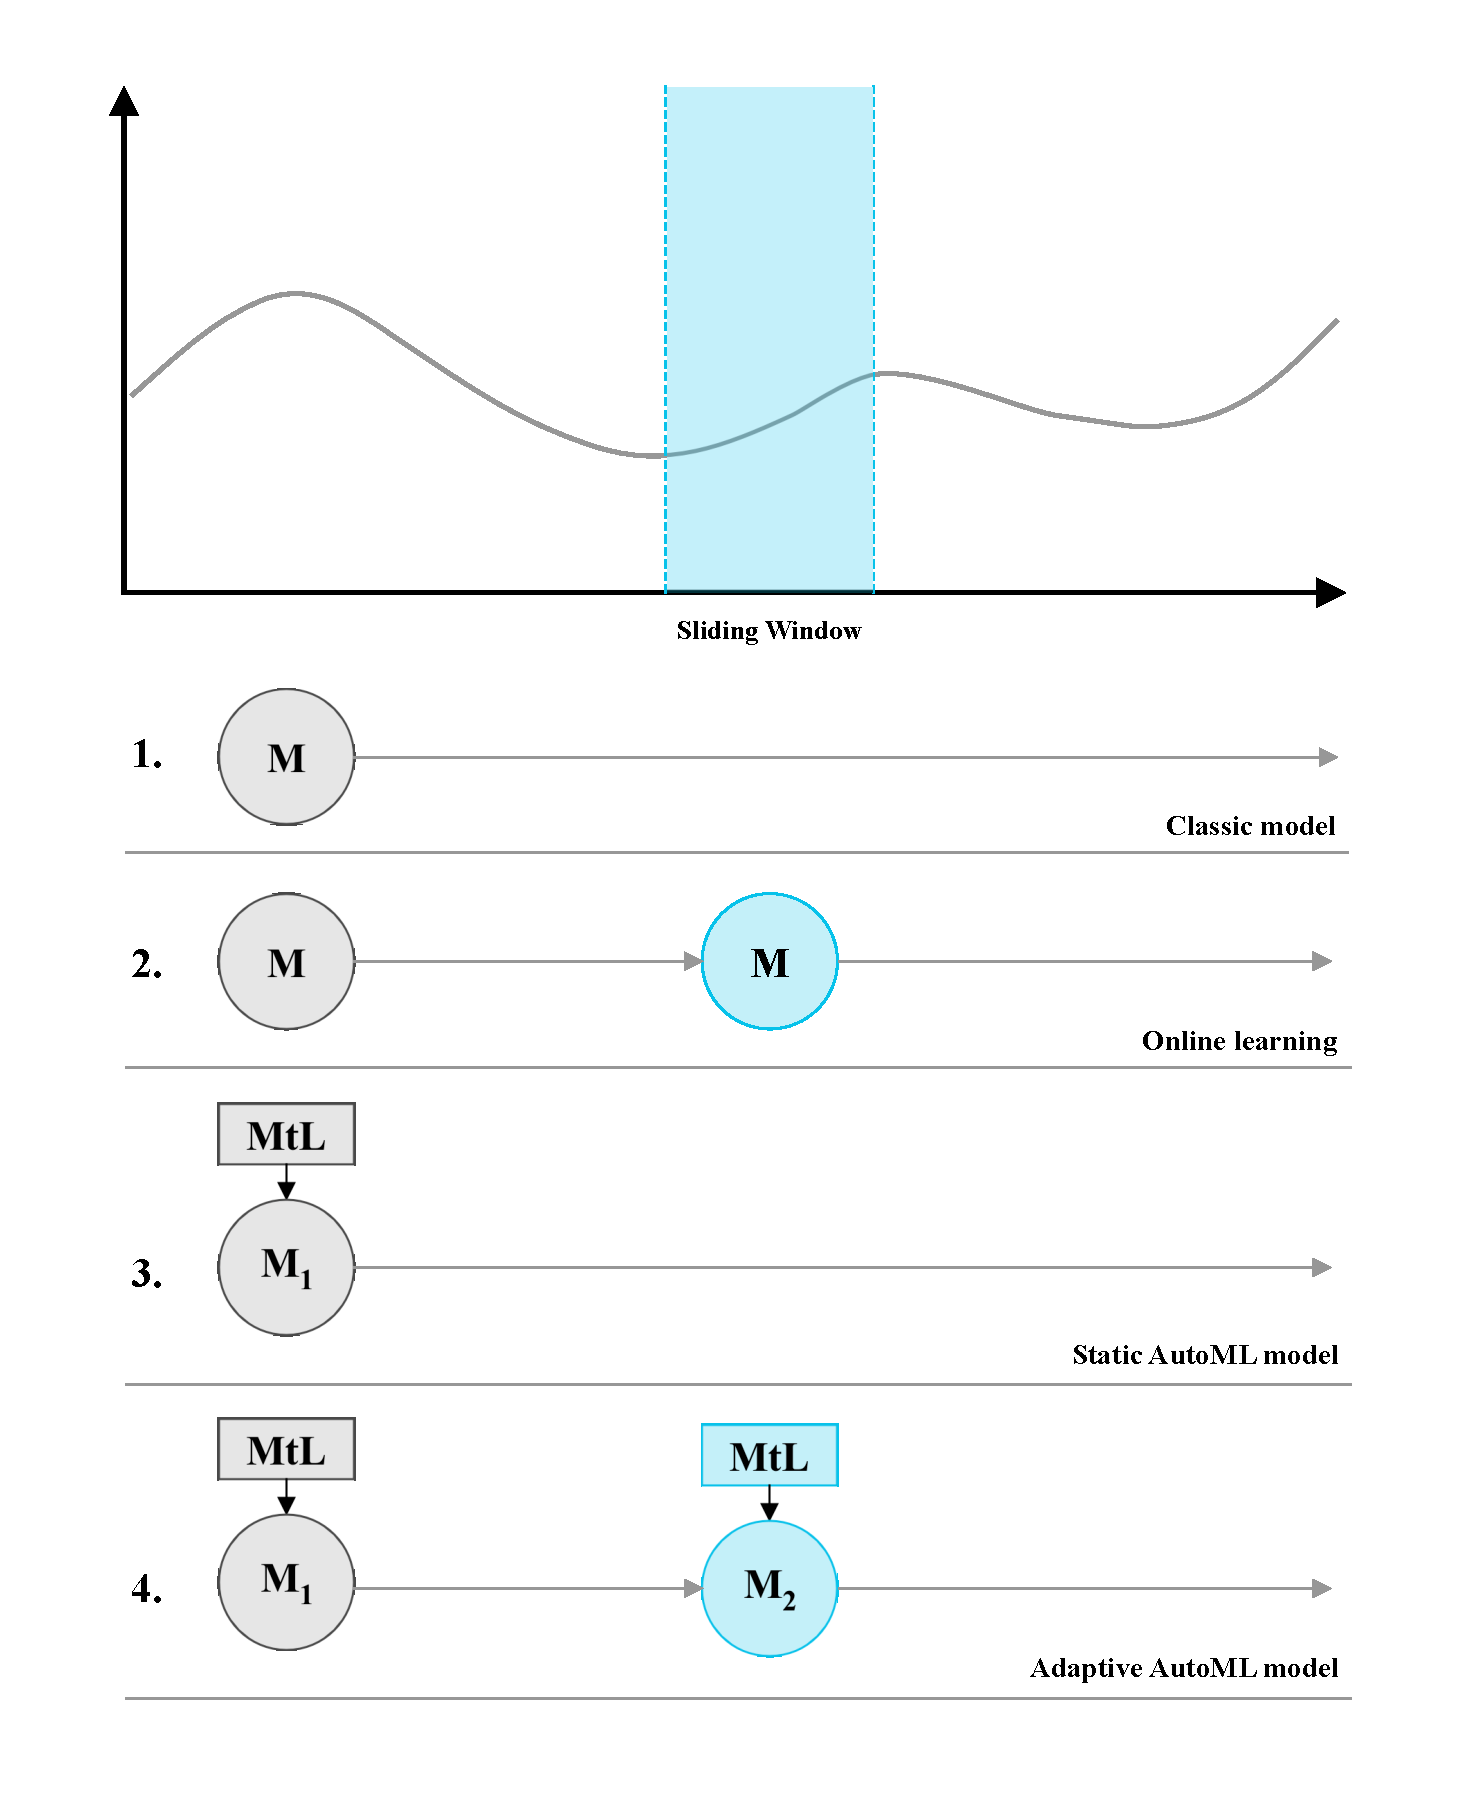
\epsfig{file=experiments.eps, width=8.5cm}
\caption{Experiment Types}
\label{fig:experiments}
\end{figure}

A visual representation of the proposed experiments types can be observed in the Figure \ref{fig:experiments}. The first two types of experiments do not involve any AutoML approach and serve as baseline for the other experiments. While the first experiment implies the usage of a model trained on a bounded part of the stream used as training data, the second experiment implies using online learning algorithms than can perform (batch) incremental learning or ensemble of those such as \textbf{Hoeffding Tree, OzaBag, OzaBoost}. The third experiment consists of using AutoFE, HPO and meta-learning to generate a meta-model or meta-learner (\textbf{MtL} in the Figure \ref{fig:experiments}) based on the meta-features of the data set and using the meta-learner to select the algorithm, its features, and hyperparameters. The fourth experiment consists of using the meta-learner over time to select the model and perhaps optimize the parameters for the next sliding window. 



The benchmark data sets will include both real and synthetic ones in order to provide verifiability and reproducibility. One of the real data sets will be the well known Airlines data sets created by the American Statistical Association which contains 120 million flights in from the United States between October 1987 and December 2008. It is usually used in literature to predict departure delays. 


The planned method to convert batch data sets into streams is by ingesting the data into Kafka \footnote{\url{https://kafka.apache.org}}, a scalable Pub/Sub broker which also has a distributed event log, and replay the log as a stream. This approach allows replaying a stream multiple times, from different points in time and at different "speeds". By replaying the stream, the time lapsing behaviour required to perform the experiments of the \textbf{RQ2} can be achieved. 

\begin{table*}[]
\renewcommand{\arraystretch}{1.25}
\caption{Weekly Time Planning and Deadlines}
\label{table:planning}
\centering
\begin{tabular}{|l|l|l|l|l|l|l|l|l|l|l|l|l|}
\hline
\textbf{Calendar Week} & \textbf{46} & \textbf{47} & \textbf{48} & \textbf{49} & \textbf{50} & \textbf{51} & \textbf{52} & \textbf{1} & \textbf{2} & \textbf{3} & \textbf{4} & \textbf{5} \\ \hline
\textbf{Module Week} & \textbf{1} & \textbf{2} & \textbf{3} & \textbf{4} & \textbf{5} & \textbf{6} & \textbf{7} & \textbf{8} & \textbf{9} & \textbf{10} & \textbf{11} & \textbf{12} \\ \hline
Research topic selection & \cellcolor[HTML]{C0C0C0}{\color[HTML]{333333} } &  &  &  &  &  &  &  &  &  &  &  \\ \hline
Literature research & \cellcolor[HTML]{C0C0C0}{\color[HTML]{000000} } & \cellcolor[HTML]{C0C0C0}{\color[HTML]{000000} } & \cellcolor[HTML]{C0C0C0}{\color[HTML]{000000} } &  &  &  &  &  &  &  &  &  \\ \hline
Draft research proposal &  & \cellcolor[HTML]{C0C0C0}\textbf{24/11} &  &  &  &  &  &  &  &  &  &  \\ \hline
Peer review research proposal &  &  & \cellcolor[HTML]{C0C0C0}\textbf{26/11} &  &  &  &  &  &  &  &  &  \\ \hline
Final research proposal &  &  & \cellcolor[HTML]{C0C0C0}\textbf{01/12} &  &  &  &  &  &  &  &  &  \\ \hline
Research and implement RQ1 &  &  & \cellcolor[HTML]{C0C0C0} & \cellcolor[HTML]{C0C0C0} & \cellcolor[HTML]{C0C0C0} &  &  &  &  &  &  &  \\ \hline
Compare models performance RQ2 &  &  &  &  &  & \cellcolor[HTML]{C0C0C0} & \cellcolor[HTML]{C0C0C0} & \cellcolor[HTML]{C0C0C0} &  &  &  &  \\ \hline
Meta-learning experiment RQ2.1 &  &  &  &  &  &  & \cellcolor[HTML]{C0C0C0} &  &  &  &  &  \\ \hline
HPO experiment RQ2.2 &  &  &  &  &  &  &  & \cellcolor[HTML]{C0C0C0}{\color[HTML]{000000} } &  &  &  &  \\ \hline
Draft research paper &  &  &  &  &  &  & & \cellcolor[HTML]{C0C0C0}{\color[HTML]{000000} } & \cellcolor[HTML]{C0C0C0}{\color[HTML]{000000} } & \cellcolor[HTML]{C0C0C0}{\color[HTML]{000000} \textbf{19/01}} &  &  \\ \hline
Final research paper &  &  &  &  &  &  &  &  &  &  & \cellcolor[HTML]{C0C0C0}\textbf{26/01} &  \\ \hline
Conference presentation &  &  &  &  &  &  &  &  &  &  &  & \cellcolor[HTML]{C0C0C0}\textbf{31/01} \\ \hline
\end{tabular}
\end{table*}

\newpage
\section{Expected results}
The expected results include:
\begin{itemize}
  \item An overview and a discussion of the possible AutoML techniques and tools that can be applied to data streams.
  \item Offline-trained AutoML models deployed for real-time predictions.
  \item Online-trained models that use the data stream both for training and evaluation data.
  \item Experiments for meta-learning, hyperparameter optimization and online AutoFE.
  \item Comparative results and interpretation.
\end{itemize}

Other possible results than can represent a valuable contribution to the open-source community and industry:
\begin{itemize}
  \item An open-source library for performing AutoML on streams.
  \item A repository with containerized experiments than can be easily reproduced.
\end{itemize}

\section{Time planning}
As shown in Table \ref{table:planning}, most of the research project time will be dedicated to the creation of the proposed and experiments and to the interpretation of the results.


% The following two commands are all you need in the
% initial runs of your .tex file to
% produce the bibliography for the citations in your paper.
\bibliographystyle{abbrv}
\bibliography{automl}  
% automl.bib is the name of the Bibliography in this case
% You must have a proper ".bib" file
%  and remember to run:
% latex bibtex latex latex
% to resolve all references
%
% ACM needs 'a single self-contained file'!
\end{document}
